\normalfont\documentclass[letterpaper,11pt]{article}
\usepackage{amsmath, amsfonts,amssymb,latexsym}
\usepackage{fullpage}
\usepackage{parskip}
\usepackage{flexisym}
\usepackage{algorithm}
\usepackage{indentfirst}
\usepackage{graphicx}
\usepackage{algorithmicx}
\usepackage{algpseudocode}
\usepackage{pythonhighlight}
\usepackage{amsmath}
\usepackage{hyperref}
\begin{document}
\setlength{\parindent}{2ex}
\newcommand{\header}{
	\noindent \fbox{
	\begin{minipage}{6.4in}
  	\medskip
  	\textbf{CS 261 - Data Structure} \hfill \textbf{Spring 2017} \\[1mm]
  	\begin{center}
    	{\Large HomeWork 6} \\[3mm]
  	\end{center}
	\today \hfill \itshape{Liangjian Chen}
	\medskip
	\end{minipage}}
}
\newcommand{\RN}[1]{%
  \textup{\uppercase\expandafter{\romannumeral#1}}%
}
\bigskip
\header

\begin{enumerate}
\item [Problem 1]\textbf{Solution:}\par
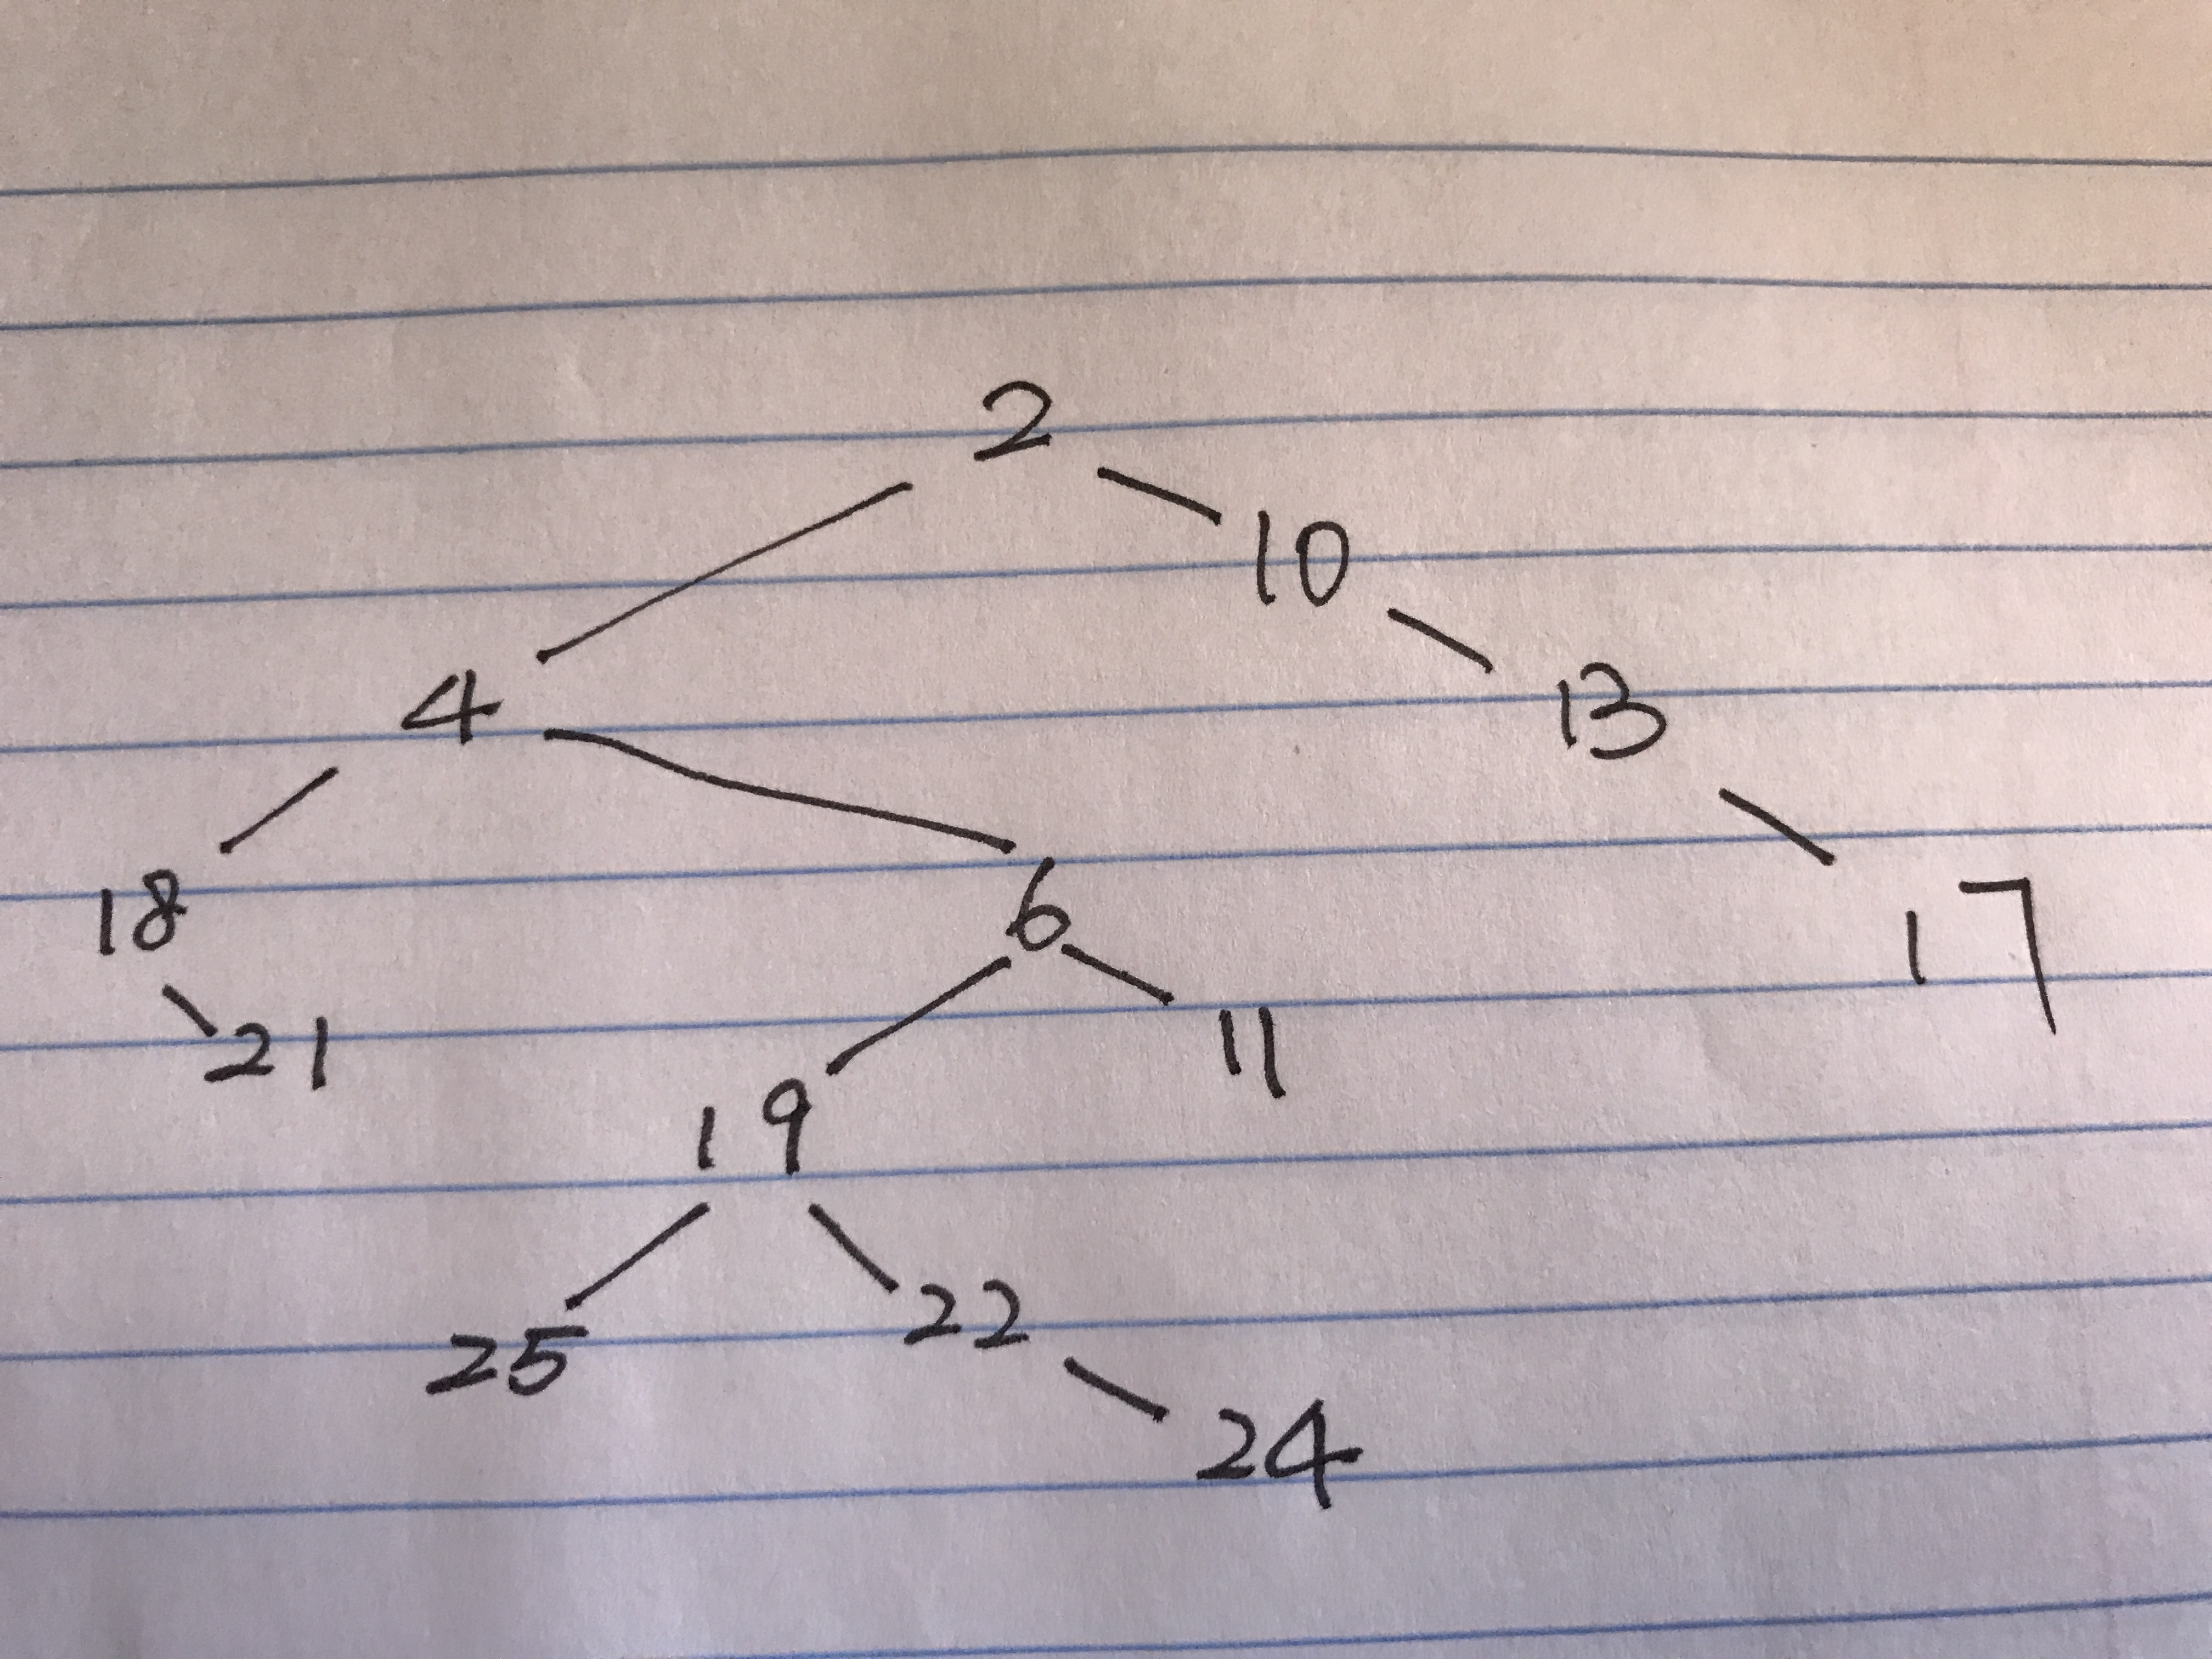
\includegraphics[width=6in]{1.JPG}\par
The query between node $24$ and node $13$.
\item [Problem 2]\textbf{Solution:}\par
$(2,0)\rightarrow(4,1)\rightarrow (18,2)\rightarrow (21,3)\rightarrow (18,2)\rightarrow(4,1)\rightarrow(6,2)\\
\rightarrow(19,3)\rightarrow (25,4)\rightarrow (19,3)\rightarrow (20,4)\rightarrow (22,5)\rightarrow(24,6)\rightarrow(22,5)\\
\rightarrow(20,4) \rightarrow(19,3)\rightarrow (6,2)\rightarrow (11,3)\rightarrow (6,2)\rightarrow(4,1)\rightarrow(2,0)\\
\rightarrow(10,1)\rightarrow (13,2)\rightarrow (17,3)\rightarrow (13,2)\rightarrow(10,1)\rightarrow(2,0)$\par
Assume 0-index, positions are 12 and 22.
\item [Problem 3]\textbf{Solution:}\par
$+-+-+$ can not occur in this sequence, because the degree of a node is at most 2, it must go up after going down, going up, going down and going up.
\item [Problem 4]\textbf{Solution:}\par
When $LCA(x,y)$ is not $x$, first step is to the $x$'s father. In the case of $LCA(x,y) = x$, if $LCA(x\text{'s left son},y)$ is $x's$ left son, go left son, otherwise right son.\par
Therefore we make LCA query at most twice.
\end{enumerate}
\end{document}
